\section{Experiments}

\subsection{Settings}

\textbf{Tasks.}
We evaluate \ourmethod on two standard benchmarks, Terminal-Bench~\citep{tbench_2025} and ARC-AGI-2~\citep{chollet2025arc}, and three open-ended optimization tasks, circle\_packing\_26 (CP26)\citep{cp26}, autocorrelation\_second (AC2)\citep{ac2}, and Anthropic's Kernel optimization task~\citep{takehome}. Together, these tasks cover agentic problem solving, abstract reasoning, and code-evolving open-ended optimization. Detailed task definitions and evaluation protocols are given in Appendix~\ref{appendix:task_metric_details}.

\textbf{Baselines.}
We group baselines into three families: single-agent inference, agent-based evolution, and procedure-based evolution. On Terminal-Bench and ARC-AGI-2, we compare against one-shot ReAct~\citep{yao2022react} and five procedure-based evolution baselines: ADAS~\citep{hu2024automated}, DGM~\citep{zhang2025darwin}, AFlow~\citep{zhang2024aflow}, SPO~\citep{xiang2025self}, and GEPA~\citep{agrawal2025gepa}. On the three open-ended tasks, we compare against two agent-based evolution baselines, Codex and Claude Code, and two procedure-based evolution baselines, OpenEvolve~\citep{openevolve} and HyperAgents~\citep{zhang2026hyperagents}. This setup lets us compare both variants of \ourmethod against systems that either keep a fixed search procedure or rely on an agent to improve artifacts directly.

\textbf{Implementation Details.}
\ourmethod is instantiated in two forms. In the procedure-based setting, a meta-agent edits the evolution procedure while leaving the task evaluator fixed. In the agent-based setting, the meta-agent steers a coding-agent harness through prompts, notes, and reusable utilities. We use Claude Code and Codex as the meta-agent interfaces, backed by Claude-Opus-4.7 and GPT-5.4 as the optimization models. For Terminal-Bench and ARC-AGI-2, candidate execution uses Gemini-3-Flash. All models are accessed through APIs. Full hyperparameter settings, round budgets, early-stopping criteria, and initialization details are given in Appendix~\ref{appendix:impl_details}.

\textbf{Metrics.}
For Terminal-Bench and ARC-AGI-2, we report task score and the first optimization round that reaches the best score. Results are summarized with Avg@3 over three independent runs. For the open-ended tasks, we report the task-native objective with Best@3 over three runs, together with the first round that reaches the best result (Best R.) and the average dollar cost per optimization round (\$/R). Exact task-specific objectives and cost computation are provided in Appendix~\ref{appendix:task_metric_details}.

\subsection{Main Results}

\begin{table*}[htbp]
\caption{
Open-ended optimization results.
Task 1/2/3 correspond to circle\_packing\_26, autocorrelation\_second, and Kernel optimization task.
Scores denote Best@3 over three runs using the model shown in the Model column, Best R. denotes the first round reaching the reported best score, and \$/R denotes the average cost per optimization round.
Arrows indicate optimization direction; \textbf{bold} and \underline{underline} mark the best and second-best scores.
}
\label{tab:open-ended-results}
\centering
\footnotesize
\setlength{\tabcolsep}{1.9pt}
\renewcommand{\arraystretch}{1.15}

\begin{tabular}{lll ccccccccc}
\toprule[1.2pt]
\multirow{2}{*}[-3pt]{\textbf{Category}}
& \multirow{2}{*}[-3pt]{\textbf{Method}}
& \multirow{2}{*}[-3pt]{\textbf{Model}}
& \multicolumn{3}{c}{\textbf{Task 1 $\uparrow$}}
& \multicolumn{3}{c}{\textbf{Task 2 $\uparrow$}}
& \multicolumn{3}{c}{\textbf{Task 3 $\downarrow$}} \\
\cmidrule(lr){4-6}
\cmidrule(lr){7-9}
\cmidrule(lr){10-12}
& &
& \textbf{Score} & \textbf{Best R.} & \textbf{\$/R}
& \textbf{Score} & \textbf{Best R.} & \textbf{\$/R}
& \textbf{Score} & \textbf{Best R.} & \textbf{\$/R} \\
\midrule[0.8pt]

\multirow{2}{*}{\makecell{Agent-Based\\Evolution}}
& Codex       & GPT-5.4
& \textbf{2.6359} & 3 & 0.82
& 0.9176 & 96 & 0.04
& 1667 & 4 & 0.96 \\
& Claude Code & Claude-Opus-4.7
& \underline{2.6305} & 50 & 0.78
& \underline{0.9438} & 44 & 0.81
& 1615 & 97 & 0.51 \\

\midrule[0.3pt]

\multirow{4}{*}{\makecell{Procedure-Based\\Evolution}}
& OpenEvolve  & Claude-Opus-4.7
& 2.6303 & 80 & 0.42
& 0.9186 & 99 & 0.67
& 2411 & 99 & 0.62 \\
& HyperAgents & Claude-Opus-4.7
& \textbf{2.6359} & 32 & 9.50
& 0.9245 & 48 & 2.83
& 7086 & 86 & 1.56 \\
& OpenEvolve  & GPT-5.4
& 2.6341 & 19 & 0.23
& 0.9118 & 74 & 0.54
& 2464 & 100 & 0.57 \\
& HyperAgents & GPT-5.4
& 2.6359 & 47 & 3.19 
& 0.9237 & 61 & 1.46
& 3015 & 98 & 1.03 \\

\midrule[0.3pt]

\multirow{3}{*}{Ours}
& \ourmethod$_{\texttt{Procedure}}$ & Claude-Opus-4.7
& \textbf{2.6359} & 4 & 1.47
& 0.9278 & 29 & 0.70
& 1803 & 55 & 1.37 \\
& \ourmethod$_{\texttt{Agent}}$ & Claude-Opus-4.7
& \textbf{2.6359} & 2 & 0.34
& \textbf{0.9459} & 99 & 1.40
& \underline{1519} & 55 & 1.27 \\
& \ourmethod$_{\texttt{Agent}}$ & GPT-5.4
& \textbf{2.6359} & 17 & 0.32
& 0.9398 & 100 & 1.31
& \textbf{1138} & 99 & 1.23 \\

\bottomrule[1.2pt]
\end{tabular}

\vspace{0.4em}
\end{table*}

\begin{table*}[htbp]
\caption{
Standard benchmark results.
Scores denote Avg@3 over three runs with Gemini-3-Flash as the execution model, and Best R. denotes the first round reaching the reported best score.
The \textbf{bold} and \underline{underline} mark the best and second-best scores.
}
\label{tab:standard-results}
\centering
\small
\setlength{\tabcolsep}{4pt}
\renewcommand{\arraystretch}{1.15}

\begin{tabular}{lll cccccc}
\toprule[1.2pt]
\multirow{2}{*}[-3pt]{\textbf{Category}}
& \multirow{2}{*}[-3pt]{\textbf{Method}}
& \multirow{2}{*}[-3pt]{\textbf{Model}}
& \multicolumn{2}{c}{\textbf{Terminal-Bench $\uparrow$}}
& \multicolumn{2}{c}{\textbf{ARC-AGI-2 $\uparrow$}} \\
\cmidrule(lr){4-5}
\cmidrule(lr){6-7}
& &
& \textbf{Score} & \textbf{Best R.}
& \textbf{Score} & \textbf{Best R.} \\
\midrule[0.8pt]

Single-Agent Inference
& ReAct $_{\texttt{Pass@1}}$ & Gemini-3-Flash
& 28.6 & --
& 21.8 & -- \\

\midrule[0.3pt]

\multirow{5}{*}{\makecell{Procedure-Based\\Evolution}}
& ADAS  & Gemini-3-Flash
& 38.6 & 7
& \underline{36.0} & 3 \\
& DGM   & Gemini-3-Flash
& \underline{44.3} & 19
& 29.8 & 5 \\
& AFlow & Gemini-3-Flash
& \underline{44.3} & 11
& 31.8 & 14 \\
& SPO   & Gemini-3-Flash
& 42.9 & 19
& 25.0 & 6 \\
& GEPA  & Gemini-3-Flash
& 41.4 & 15
& 22.5 & 13 \\

\midrule[0.3pt]

Ours
& \ourmethod$_{\texttt{Procedure}}$ & Gemini-3-Flash
& \textbf{53.8} & 7
& \textbf{47.0} & 12 \\

\bottomrule[1.2pt]
\end{tabular}

\vspace{0.4em}
\end{table*}

\textbf{Overall performance.}
Tables~\ref{tab:open-ended-results} and~\ref{tab:standard-results} show that \ourmethod consistently improves agentic evolution across both open-ended optimization and fixed benchmarks.
On the open-ended tasks, \ourmethod achieves the best or tied-best result on all three tasks, while also improving the speed or stability with which strong candidates are found.
In particular, on the Kernel optimization task, \ourmethod achieves 1138 cycles within 100 iterations, which is, to our knowledge, the best reported result under the same iteration budget.
This suggests that the harnessed meta-editing loop improves how evolution uses feedback over time, rather than merely increasing the number of candidate attempts.
On standard agentic and reasoning benchmarks, \ourmethod also improves procedure-based evolution over strong fixed-loop baselines.
The gains are consistent across both Terminal-Bench and ARC-AGI-2, yielding a 26\% relative improvement over the strongest baseline on average.
Together, these results support the central claim that mechanism-level intervention can benefit both open-ended optimization and benchmark-driven agentic evolution.

\textbf{Improvement through optimization-time reasoning.}
The gains on Table \ref{tab:standard-results} come with a higher per-round optimization cost.
\ourmethod costs about three times as much as procedure-based baselines on these benchmarks.
This means that \ourmethod improves performance by scaling the reasoning and deliberation used during optimization, and supports our view that increasing the budget of the evolution process is a useful axis for improving agentic evolution.

\textbf{Cost analysis and agentic behavior.}
The open-ended tasks reveal that cost is not solely determined by whether a method is agent-based or procedure-based.
Agent-based evolution can remain cost-competitive when implemented through coding-agent interfaces with prompt caching and persistent contexts.
\ourmethod$_{\texttt{Agent}}$ maintains low per-round cost: 0.34--0.32 on \textit{circle\_packing\_26}, 1.40--1.31 on \textit{autocorrelation\_second}, and 1.27--1.23 on Kernel optimization.
By contrast, procedure-based methods can become expensive in long-horizon optimization by repeatedly constructing large prompts over an expanding search history without comparable caching, as visible in HyperAgents' higher per-round cost on Task 1 and Task 2.

At the same time, direct coding agents show why agent freedom alone is insufficient for reliable evolution.
Even with prompts encouraging long-horizon search, coding agents often stop early once local improvements become difficult, as seen in the early best rounds of Codex on Task 1 and Task 3.
This suggests that an agent's internal stopping decision can conflict with the external evolution budget.
\ourmethod addresses this by placing the coding agent inside an explicit evolution harness, where rounds, candidate records, and evaluation feedback are maintained outside the agent's local decision loop.


\subsection{Evolution Dynamics}

\begin{figure}[htbp]
\centering
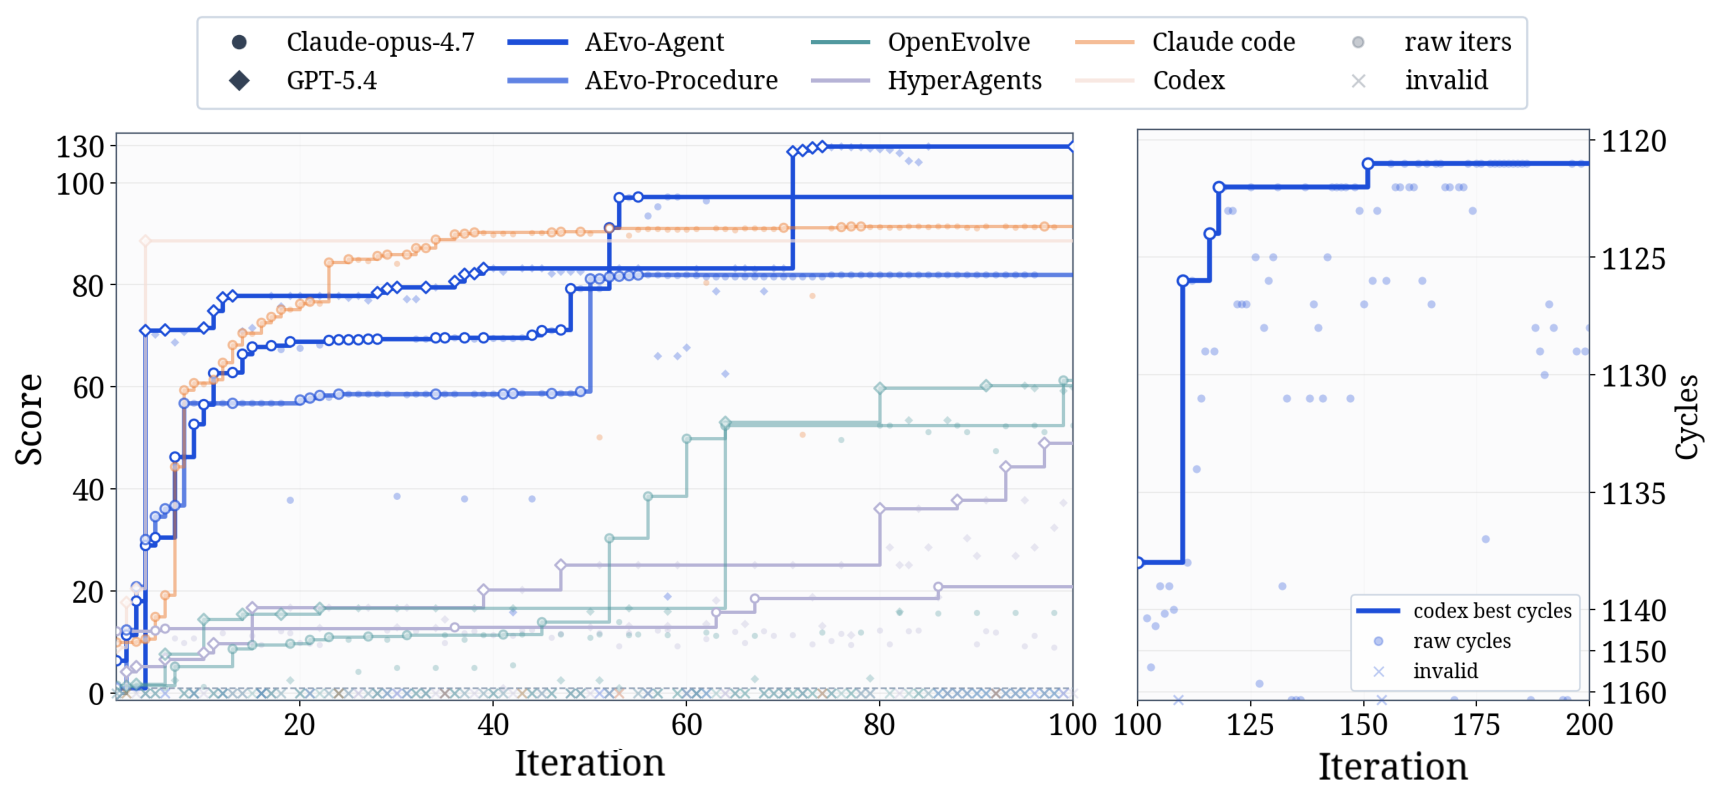
\includegraphics[width=\linewidth]{images/Figure-3.pdf}
\caption{
Evolution trajectories on the \textit{Kernel optimization} task.
The left panel compares eight methods over the first 100 iterations, where blue curves denote \ourmethod variants.
The y-axis reports the normalized score induced by cycle reduction, so higher is better; raw iterations and invalid evaluations are shown as scattered markers.
The right panel extends the \ourmethod run from 100 to 200 iterations and reports raw cycles, where lower is better.
}
\label{fig:evolution-dynamics}
\end{figure}

\textbf{Revising evolution after plateaus.}
As shown in Figure~\ref{fig:evolution-dynamics}, procedure-based methods such as OpenEvolve and HyperAgents tend to flatten once their current selection or mutation strategy stops producing useful candidates.
In contrast, \ourmethod can revise the mechanism that drives subsequent evolution.
When progress stalls or repeated failures appear, these signals become process-level feedback: the meta-agent can adjust the procedure, directive, or reusable search context, producing step-wise improvements after plateaus.
This is visible in the late-stage jump that leads to the best 100-round result.

\textbf{Using the evolution budget effectively.}
Direct coding agents can obtain strong early gains through internal simulation, execution, and debugging, but they may stop early once local progress becomes difficult.
\ourmethod avoids tying progress to the agent's local stopping decision by maintaining explicit rounds, candidate records, and evaluation feedback outside the agent context.
This allows the external evolution budget to be used more consistently.

\textbf{Scaling beyond early gains.}
The right panel extends Codex-based \ourmethod from 100 to 200 iterations.
The best result improves from 1138 to 1121 cycles, showing that \ourmethod continues to benefit from additional rounds rather than saturating after an early strong candidate.
Overall, the trajectories suggest that agent flexibility is useful, but reliable long-horizon improvement requires a harness that preserves global evidence and enables mechanism-level correction.


\subsection{Ablation Study}

Table~\ref{tab:ablation} (Appendix) ablates two key components of \ourmethod$_{\texttt{Agent}}$ on the Kernel optimization task. The full system completes the 100-round budget without reward hacking and reaches the best valid result of 1138 cycles. Removing meta-agent skills does not lead to reward hacking, but it substantially weakens long-horizon search: the best run only reaches 1407 cycles, and the runs do not consistently sustain the full budget. Removing the evolution harness is even less reliable. Although one run finds a strong 1167-cycle solution, two of the three runs enter reward-hacking trajectories and fail to produce valid cycle results. These results suggest that the skills mainly support sustained and effective meta-intervention, while the harness provides the protected evaluation boundary and structured evolution context needed to keep agentic search aligned with the true objective.

\subsection{Case Study}

We examine two representative trajectories to illustrate how \ourmethod uses accumulated evidence to revise the evolution process.
The first case studies procedure evolution on ARC-AGI-2, while the second studies an external optimizer-discovery trajectory that produced a public pull request to the Modded-NanoGPT benchmark.

\begin{figure}[t]
    \centering
    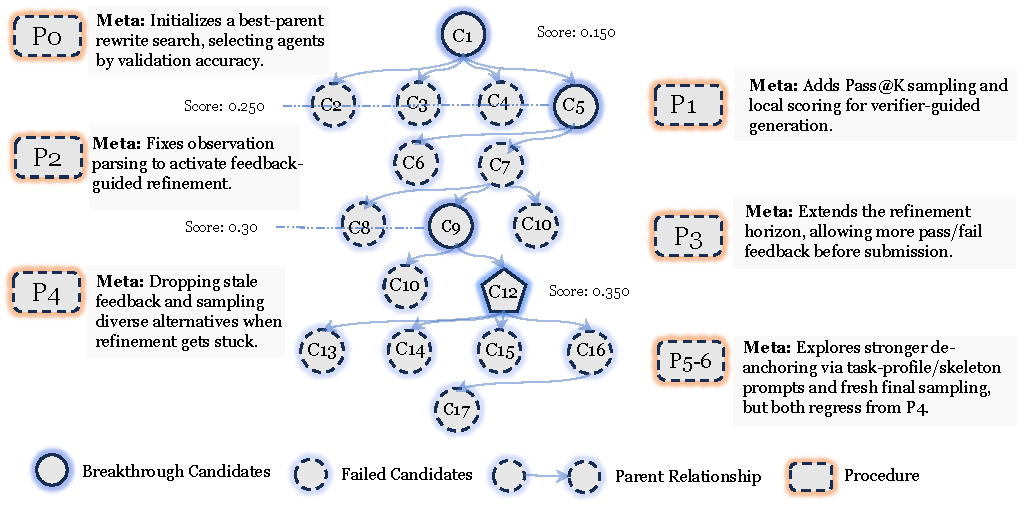
\includegraphics[width=1\linewidth]{images/case_study.pdf}
    \caption{
    Case study of procedure evolution on an ARC-AGI-2 task.
    Each $P$ denotes a procedure produced or revised by the meta-agent, and each $C$ denotes a candidate agent generated by the current procedure.
    Solid nodes are breakthrough candidates, dashed nodes are failed candidates, and arrows indicate parent relationships.
    The meta-agent improves the search process by changing the procedure across stages, while failed candidates provide feedback for later interventions.
    }
    \label{fig:case-study}
\end{figure}

\paragraph{Procedure evolution on ARC-AGI-2.}
Figure~\ref{fig:case-study} illustrates how \ourmethod performs meta-intervention during procedure-based evolution on an ARC-AGI-2 task.
Starting from $P_0$, the meta-agent initializes a best-parent rewrite procedure that selects candidate agents by validation accuracy.
This first produces an initial breakthrough candidate $C_1$, but subsequent variants expose several failure modes in observation parsing and refinement.
The meta-agent then revises the procedure rather than continuing the same search blindly: $P_1$ adds Pass@K sampling and local scoring for verifier-guided generation, $P_2$ fixes observation parsing to activate feedback-guided refinement, and $P_3$ extends the refinement horizon to use more pass/fail feedback before submission.
When the search becomes stuck, $P_4$ drops stale feedback and samples more diverse alternatives, leading to a stronger candidate.
Later interventions $P_{5}$--$P_{6}$ explore stronger de-anchoring through task-profile and skeleton prompts, but these regress from $P_4$.
This example shows that failed candidates are not merely discarded; they become process-level evidence that helps the meta-agent decide how to revise the future evolution procedure.
Additional evolved procedures, optimized agent harnesses, and task-level analyses are provided in Appendix~\ref{appendix:opt_procedure} and Appendix~\ref{appendix:opt_harness}.

\paragraph{External auto-research on optimizer discovery.}
Figure~\ref{fig:nanogpt-case-study} shows a second case study on the Modded-NanoGPT Track-3 optimizer-discovery benchmark, where the goal is to minimize the first training step at which a fixed nanoGPT setup reaches a validation-loss target under a statistical test.
This trajectory did not improve through a smooth local hyperparameter sweep.
Early rounds first separated infrastructure failures from optimizer evidence, then found that learning-rate schedule geometry was the first large lever.
When the evaluator shifted from single-seed crossing to a multi-seed mean objective, the search problem changed: strong candidates had to move the aggregate validation curve rather than only make one seed cross early.

The search then reached a local basin around a PR321-style SOAP-Muon stack.
A strong local candidate combined a Muon schedule near 2875 steps, Muon schedule power near 1.183, paired norm-gain initialization, and EMA-Nesterov lookahead strength 0.325, but nearby sweeps mostly shifted the bottleneck between seeds.
The decisive intervention was to change the mechanism family.
The meta-agent adopted a radius-pin-aware stack consisting of Tail-EMA evaluation readout, RowFloor, and post-pin Cautious Weight Decay, motivated by the observation that ordinary magnitude changes are erased by the radius pin whereas readout changes, row/shape changes, and post-pin anisotropy can survive.
Controlled ablations showed that this family was additive, and a final readout calibration, \texttt{TAILEMA\_TAU}=120 with \texttt{TAILEMA\_LAMBDA}=0.65, produced the best local candidate.
The resulting public PR \#331 to \href{https://github.com/KellerJordan/modded-nanogpt/pull/331}{KellerJordan/modded-nanogpt} first satisfies the benchmark's $n=8$ formal statistic at 2660 steps, with mean validation loss 3.27857375 and $(3.28-\mathrm{mean})\sqrt{8}=0.00403404$.

\begin{figure}[t]
    \centering
    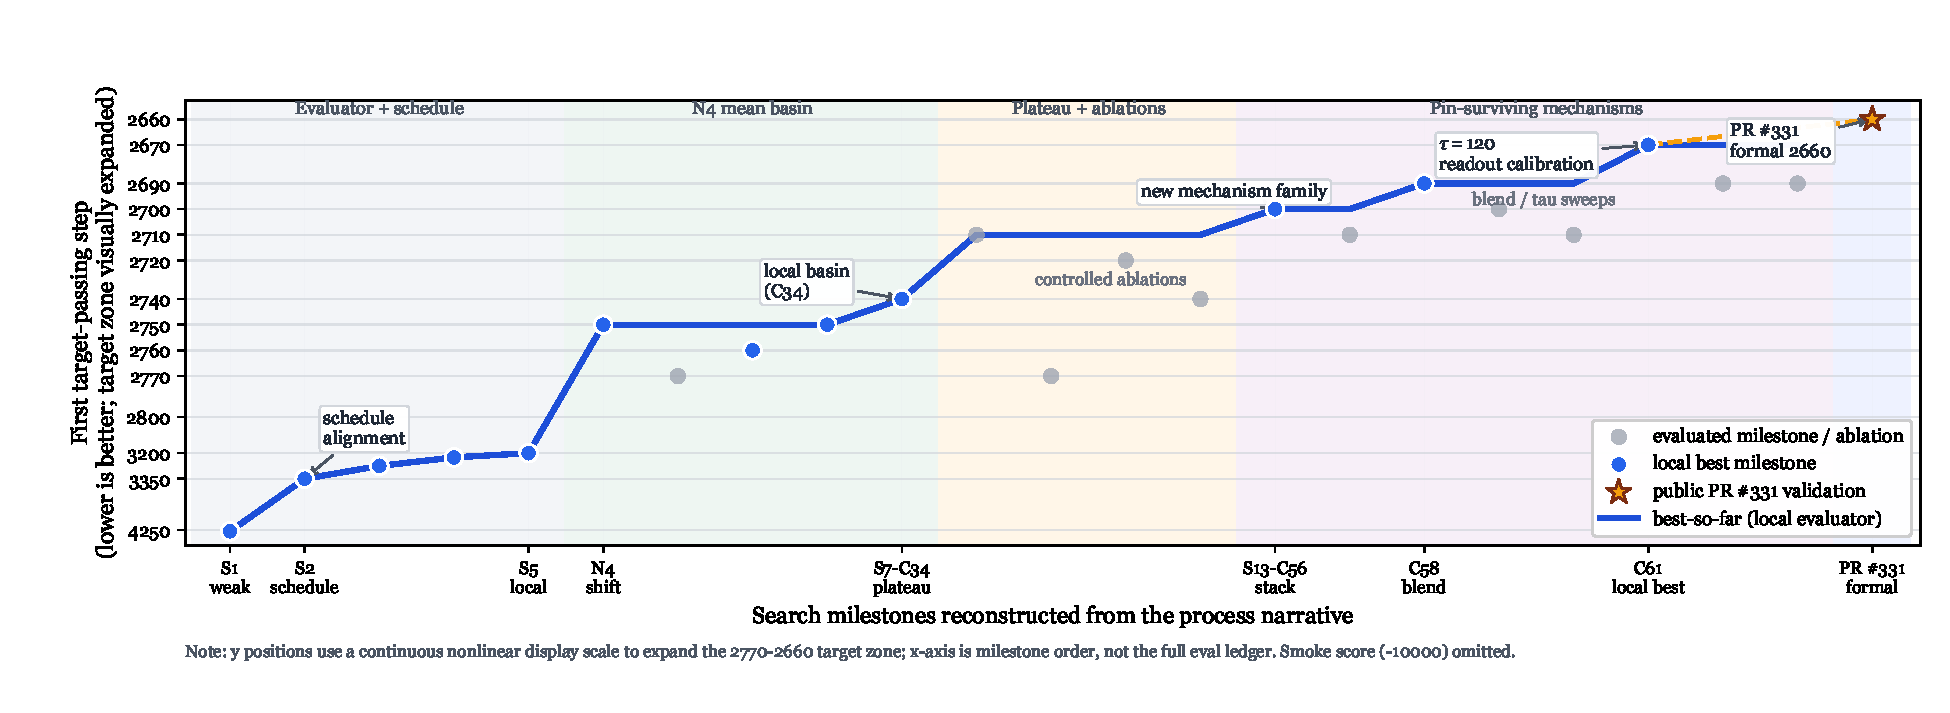
\includegraphics[width=1\linewidth]{images/nanogpt_evolve_case_study_georgia_clean_v2.pdf}
    \caption{
    Case study of external auto-research on the Modded-NanoGPT Track-3 optimizer-discovery benchmark.
    The x-axis shows reconstructed search milestones rather than the full evaluation ledger.
    The y-axis reports first target-passing training steps, where lower is better; the visual scale is continuous but nonlinear to expand the target zone from 2770 to 2660 steps.
    The trajectory first improves through evaluator grounding and schedule alignment, then plateaus around a PR321-style SOAP-Muon basin, and finally improves after the meta-agent switches to a radius-pin-surviving mechanism family.
    The final public PR \#331 validates the local trajectory under the benchmark's $n=8$ formal statistic.
    }
    \label{fig:nanogpt-case-study}
\end{figure}

\FloatBarrier
